\documentclass[11pt]{article}

\usepackage{amssymb,amsmath}
\usepackage{times,psfrag,epsf,epsfig,graphics,graphicx,caption}
\usepackage{alltt}
\usepackage{sverb}
\usepackage{verbatim}
\usepackage{enumitem}
\usepackage{algorithm}
\usepackage{algorithmic}

\begin{document}
\date{}

\title{CSCI 232: Assignment 2}

\author{William Jardee}

\maketitle


\section*{Problem 1}
Give the heap that results when the keys E A S Y Q U E S T I O N are inserted in that order into an initially empty max-heap.\\\\

Assuming that the heap will not throw out any duplicates; \\

\parbox{0}{ 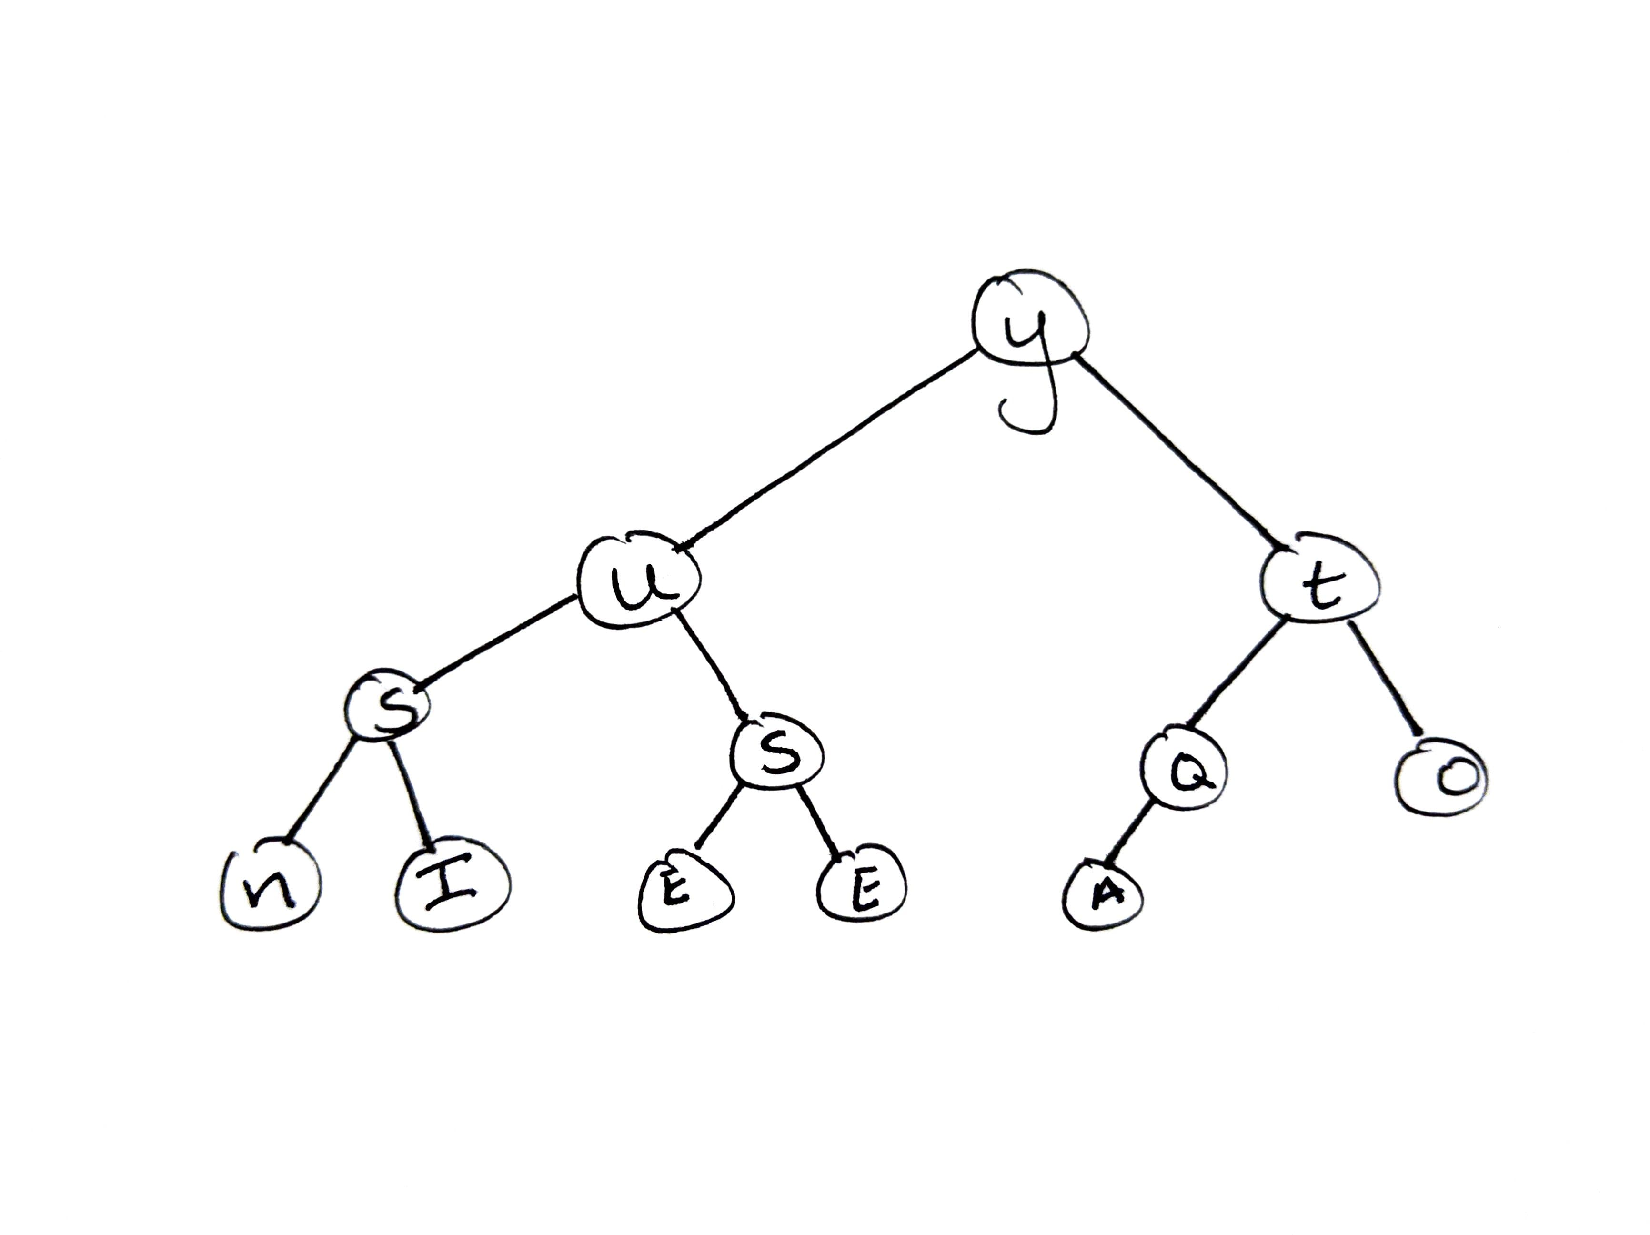
\includegraphics[width = 300pt]{Homework_2/max_heap(1).pdf}}\\
The drawn diagram follows the rule that each node can only have children that are equal to or less than them. The diagram also follows the rule of adding new nodes left to right.
\newpage

\section*{Problem 2}
The simplest solution would be to keep a max-heap that contains k elements. Every time you wish to add a new element, you add it like normal to the heap, holding a total of k+1 terms now. After the element is added, take the smallest node, the one lowest on the hierarchy, and set it equal to null. This method only keeps the very top of the heap and discards everything else. Now you run every element in your very large data set through this method and you'll be left with the max k elements.\\\\
\textit{I am going to assume you meant how will you use a max-heap to solve this, as using a min-heap makes little sense to find the maximum values. If you are fully set on using a min-heap, do the same process but multiply each value by -1 and use a min-heap.}

\newpage

\section*{Problem 3}
I'm not sure how to elaborate on this code, its pretty straight forward. I did use a ``hashtable'' to build my dictionary. There were a couple helpful reddit posts that lead me in the right direction for implementing a dictionary where the keys were Integers (thus the hashtable). For some reason the SET wouldn't let me, I assume the structure of the SET/map requires you to  have Strings as inputs. After I submit all the assignments I have due this week I'm going to read up on all that.\\
\begin{center}
\includegraphics[width = 400pt]{Homework_2/Question3.pdf}
\end{center}
\textit{I also included a .txt of the code in case you need to copy it, but latex was acting up with formatting inputed text documents, so I just brought in a pdf instead.}

\newpage

\section*{Problem 4}
\textit{A question wasn't directly asked, so I will assume you are wondering the best ways to match up all the nuts and bolts.}\\

There are two obvious solutions that pop out right away. One quite a bit better than the other. 

\begin{enumerate}
    \item If you lay the two sets of nuts and bolts out like randomly ordered arrays, then we can just treat this problem like trying to match pairs in two arrays of integers (comparables). If you grab the first element in array a, you can go item by item through array b and check if they match. If they match you can pair up both items and delete them from both arrays. Once you have the match, move onto the next item in a. This is a brute force method with time $O(n^2)$. It works, but is boring.
    \item Another solution would be to go through and sort as you go. As you go through array a and check against array b, if the two don't match you move the item in b into another group, either larger or smaller than the item from a. As we continue to find pairs, the collection of groups slowly gets ordered and we have to check less and less values as the legs start to contain smaller number of values. Ultimately what we're aiming to build is a semi-ordered heap. This doesn't work like a min or max heap, but instead more like a binary heap, where values are less on the left and greater on the right. The time comes out to $O(n lg(n))$. The downside of this approach is if we have a small group. When the group size is very small, the upfront cost of sorting each value into a proper leg out weighs the benefits that we gain for a small hand full of other values. 
\end{enumerate}

\newpage
\section*{Inputed .txt file that didn't want to format:}
\input{Homework_2/Question 3.txt}

\end{document}
